%% ===================================================================
%% Why a Perfect AUC Is Insufficient
%% IEEE conference format (IEEEtran). Compile: pdflatex paper (x2)
%%
%% Figures are in ./figures and are produced by
%%     python scripts/make_figures.py saturation pipeline 7
%% from the project repository. Every number quoted in the text is
%% read from results/report_numbers.json, which the analysis scripts
%% write; none is transcribed by hand.
%% ===================================================================
\documentclass[conference]{IEEEtran}
\IEEEoverridecommandlockouts

\usepackage{cite}
\usepackage{amsmath,amssymb}
\usepackage{graphicx}
\usepackage{booktabs}
\usepackage{url}
\usepackage[hidelinks]{hyperref}

\def\BibTeX{{\rm B\kern-.05em{\sc i\kern-.025em b}\kern-.08em
    T\kern-.1667em\lower.7ex\hbox{E}\kern-.125emX}}

\begin{document}

\title{Why a Perfect AUC Is Insufficient: Bandwidth-Dependent Margin Loss
in Ultra-Wideband Microwave Bone-Fracture Detection}

\author{
\IEEEauthorblockN{Kavin S., Balaji V., Kanishka A., Lakshmanan A.}
\IEEEauthorblockA{\textit{Department of Medical Electronics} \\
\textit{Velalar College of Engineering and Technology}\\
Erode, Tamil Nadu, India}
\and
\IEEEauthorblockN{Shalini E.}
\IEEEauthorblockA{\textit{Department of Medical Electronics} \\
\textit{Velalar College of Engineering and Technology}\\
Erode, Tamil Nadu, India}
}

\maketitle

\begin{abstract}
Simulation studies of microwave fracture detection routinely report
near-perfect classification. We show that such a figure can be
uninformative, and that reporting it alone can support a materially wrong
engineering decision. Using a full-wave finite-difference time-domain model
of a layered forearm, we generated 192 ultra-wideband (3--11\,GHz)
acquisitions spanning eight simulated specimens, four soft-tissue overlay
thicknesses and six fracture states, and scored each under three independent
instrument-error realisations. Fractured and intact limbs separate by
40.8\,dB with no overlap, giving an area under the receiver operating
characteristic curve (AUC) of 1.0000. Because that statistic is saturated,
we re-scored the identical 192 cells over restricted frequency windows, a
controlled manipulation requiring no further electromagnetic simulation.
Removing 3.00--4.35\,GHz reduced the class separation from 40.8\,dB to
17.9\,dB, more than half, \emph{while the AUC remained exactly 1.0000}. The
metric registered none of the loss. We identify the mechanism as a loss of
range resolution, 3.67\,mm to 4.42\,mm, which prevents migration from
collapsing a layered-interface artefact and converts it into a
specimen-dependent false alarm. We argue that any study reporting a
saturated classification statistic should report the underlying margin in
decibels alongside it, and we quantify what that practice would have changed
here.
\end{abstract}

\begin{IEEEkeywords}
microwave imaging, ultra-wideband, bone fracture, FDTD, detection margin,
area under curve, model evaluation
\end{IEEEkeywords}

\section{Introduction}

Fracture diagnosis is dominated by projection radiography and computed
tomography, both of which deliver ionising radiation and require fixed
clinical infrastructure. This makes them poorly suited to repeated
monitoring of healing, and unavailable at the point of injury. Microwave
imaging is an attractive alternative because bone and the surrounding soft
tissue differ substantially in permittivity, and because a fracture filled
with blood presents a strong dielectric discontinuity against cortical bone
\cite{gabriel}.

The physical difficulty is that the water content creating the contrast also
creates the loss. The interrogating signal must cross skin, fat and muscle
twice, and attenuation rises steeply with frequency. The usable band is
therefore a compromise between range resolution, which improves with
bandwidth, and penetration, which degrades with it.

Simulation is the natural first instrument for exploring that compromise,
and a large body of such work reports excellent discrimination between
fractured and intact bone. This paper is concerned with how those results
are \emph{evaluated} rather than with whether they are achievable. Our
starting observation is that a classifier which separates two classes
completely produces an AUC of exactly 1.0000, and that this value is a
\emph{ceiling}. Once reached, the statistic cannot distinguish a system with
an enormous margin from one that is close to failing. Any subsequent
degradation, whether from reduced bandwidth, a harsher error model or a more
difficult anatomy, is invisible until it becomes severe enough to cause an
actual misclassification.

We make three contributions.

\begin{enumerate}
\item A full-wave study of ultra-wideband fracture detection comprising 192
acquisitions across a factorial design, analysed under a statistical plan
fixed before the data were examined, including leave-one-specimen-out
validation and a bootstrap that resamples specimens rather than
measurements.
\item A controlled demonstration that a saturated AUC conceals the loss of
more than half the detection margin. Because the manipulation is applied to
the stored full-band response of the same solved cells, bandwidth is varied
with everything else held exactly constant.
\item Identification of the mechanism, and a concrete reporting
recommendation whose effect on our own engineering decisions we quantify.
\end{enumerate}

\section{Method}

\subsection{Tissue model}
Permittivity and conductivity follow the Gabriel four-Cole--Cole
parameterisation \cite{gabriel}. A time-domain solver cannot integrate a
Cole--Cole response directly, because the fractional-power relaxation has no
finite-order time-domain equivalent, so each tissue is refitted to a
two-pole Debye model over 3--11\,GHz. The worst deviation across all seven
tissues is 0.23\,\%, and every relaxation time is checked to exceed the
solver time step.

\subsection{Phantom and experiment design}
The phantom is a layered forearm: skin (2.0\,mm), fat (3.0\,mm), muscle
(1.0\,mm), near cortical wall (4.0\,mm), marrow (10.0\,mm) and far cortical
wall (4.0\,mm), with the antenna at a 12\,mm standoff. A soft-tissue overlay
of 0, 3, 6 or 10\,mm spans anatomical variation. The fracture is a
rectangular blood-filled kerf in the near cortex of width 0.2, 0.4, 1.0 or
2.0\,mm, with an additional oblique state.

Eight specimens are drawn from a variation model perturbing cortical wall
thickness and overlay, giving a factorial matrix of
$8 \times 4 \times 6 = 192$ acquisitions. Without this between-specimen
variation the leave-one-specimen-out analysis would be vacuous, because
there would be nothing to leave out.

\subsection{Forward model and the inverse crime}

\begin{table}[t]
\caption{Separation of forward and inverse models}
\label{tab:crime}
\centering
\footnotesize
\begin{tabular}{@{}lll@{}}
\toprule
 & \textbf{Forward (data)} & \textbf{Inverse (image)} \\
\midrule
Physics & dispersive FDTD & homogeneous migration \\
Tissue & 6 layers, Debye & one scalar $\epsilon_{\mathrm{avg}}$ \\
Geometry & known kerf, cortex & not supplied \\
Grid & 0.2\,mm FDTD cells & independent grid \\
Error & injected & blind \\
\bottomrule
\end{tabular}
\end{table}

If the model generating the data and the model reconstructing the image
share assumptions, reconstruction always succeeds and the result is
circular. Table~\ref{tab:crime} lists the structural separations used to
avoid this. The reconstructor receives a matrix of complex $S_{11}$ values
and nothing else: not the permittivity profile, the bone geometry, the
fracture position or the noise realisation.

Data are generated with gprMax \cite{gprmax} on a 0.2\,mm grid in two
dimensions (TM$_z$). An independent analytic layered-medium model, fast
enough for development, is used only to build and unit-test the processing
chain; every result reported here comes from the full-wave solver.

\subsection{Processing chain}
Figure~\ref{fig:pipeline} shows acquisition through detection. The antenna
steps along the bone axis through 61 positions at 1\,mm spacing,
transmitting and receiving at each, giving one reflection coefficient per
position per frequency. Empty-scene subtraction removes the antenna
response; a selective singular-value decomposition removes the layered
clutter; Kirchhoff migration focuses the residual scattering back to its
origin; and a scalar peak-over-noise metric scores the result in decibels.

One parameter required revision. A common recommendation is to discard the
first two or three singular components. Measured on two independent targets,
this destroys the fracture signature along with the clutter. We instead
discard a component only if, after migration, its energy spans more than
half the scan aperture, which is the signature of a layered interface rather
than a localised scatterer.

\begin{figure*}[t]
\centering
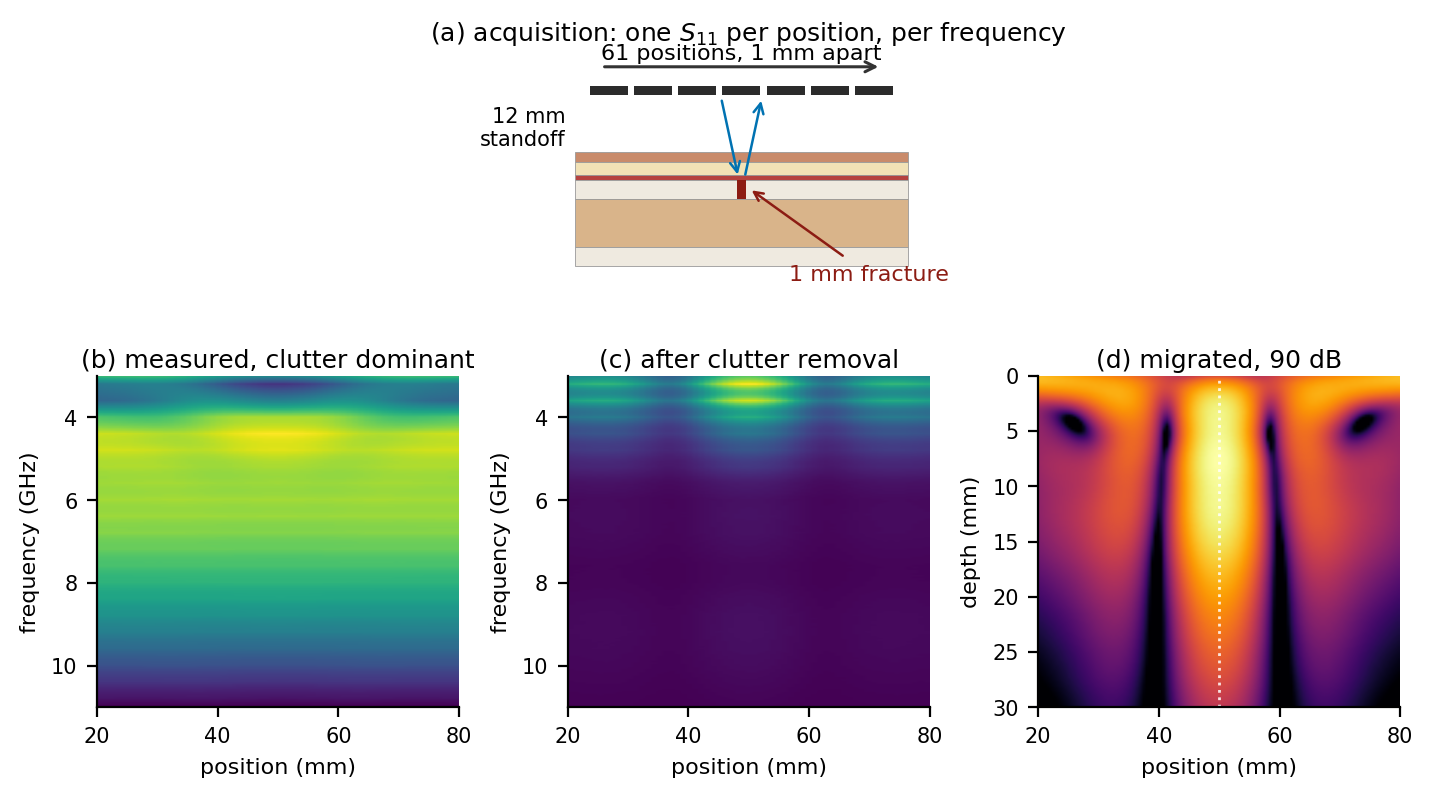
\includegraphics[width=0.98\textwidth]{figures/pipeline_paper.png}
\caption{Acquisition and processing. (a)~The antenna steps along the bone
axis at 12\,mm standoff, transmitting and receiving at each of 61 positions.
(b)~The measured response after empty-scene subtraction, dominated by
layered clutter; the fracture is present and invisible. (c)~After selective
singular-value removal, the local scattering remains. (d)~Migration focuses
it to the true position (dotted). Panels (b)--(d) are solver output for a
1\,mm fracture under 6\,mm of overlay.}
\label{fig:pipeline}
\end{figure*}

\subsection{Instrument error}
Receiver noise, cable phase drift, stage jitter and standoff variation are
injected \emph{after} the forward solve. One electromagnetic solution
therefore yields several independent ``remounts'', which is both cheaper and
physically correct, since a remount perturbs the instrument rather than the
anatomy. Three realisations per acquisition give 576 scores.

\subsection{Statistical analysis plan}
The plan was fixed before the data were examined. Two points require care.
The detector has no fitted parameters, so the only trained quantity is the
decision threshold; leave-one-specimen-out validation is therefore applied
to the threshold rather than to the detector. The bootstrap resamples
\emph{specimens}, not measurements, because twenty-four acquisitions from
one bone are not twenty-four independent observations and resampling them
would give an interval several times too narrow. Permutation labels are
shuffled within specimen for the same reason.

\section{Results}

\subsection{Detection performance}

\begin{table}[t]
\caption{Detector score distributions, 576 scores}
\label{tab:dist}
\centering
\footnotesize
\begin{tabular}{@{}lrrrr@{}}
\toprule
\textbf{Class} & \textbf{n} & \textbf{Min} & \textbf{Median} & \textbf{Max} \\
\midrule
Intact & 96 & 8.8 & 19.3 & \textbf{27.7} \\
Fractured & 480 & \textbf{68.5} & 89.9 & 104.8 \\
\bottomrule
\end{tabular}
\end{table}

Table~\ref{tab:dist} gives the raw distributions. The classes are separated
by \textbf{40.8\,dB with no overlap}, a factor of 110 in amplitude. The AUC
is 1.0000 at every overlay thickness and every fracture width, with a
bootstrap 95\,\% interval over specimens of 1.000--1.000 and a permutation
$p$ of 0.001, the floor for 1000 shuffles. Leave-one-specimen-out validation
of the threshold gives sensitivity 0.9979 (Wilson 0.988--1.000) and
specificity 1.0000 (0.962--1.000). Repeatability across remounts is
ICC(1,1) $=$ 0.9979.

A perfect AUC ordinarily indicates leakage between training and test data
rather than a genuine result, and was treated as such. Inspection of the
distributions excludes that explanation: the gap is real, and its structure
follows physical prediction. The weakest fractured cases are the narrowest
kerf under the thickest overlay, and the strongest intact cases also occur
at the thickest overlay. A leak would not order itself by physical
difficulty.

\subsection{Bandwidth-dependent margin loss}

\begin{table}[t]
\caption{The same 192 cells, re-scored over restricted bands}
\label{tab:band}
\centering
\footnotesize
\begin{tabular}{@{}lrrrr@{}}
\toprule
\textbf{Window} & \textbf{BW} & \textbf{Res.} & \textbf{AUC} &
\textbf{Sep.} \\
\midrule
3.00--11.0\,GHz & 8.00\,GHz & 3.67\,mm & 1.0000 & \textbf{40.8\,dB} \\
4.35--11.0\,GHz & 6.65\,GHz & 4.42\,mm & 1.0000 & \textbf{17.9\,dB} \\
5.00--11.0\,GHz & 6.00\,GHz & 4.90\,mm & 1.0000 & 16.0\,dB \\
\bottomrule
\end{tabular}
\end{table}

\begin{figure*}[t]
\centering
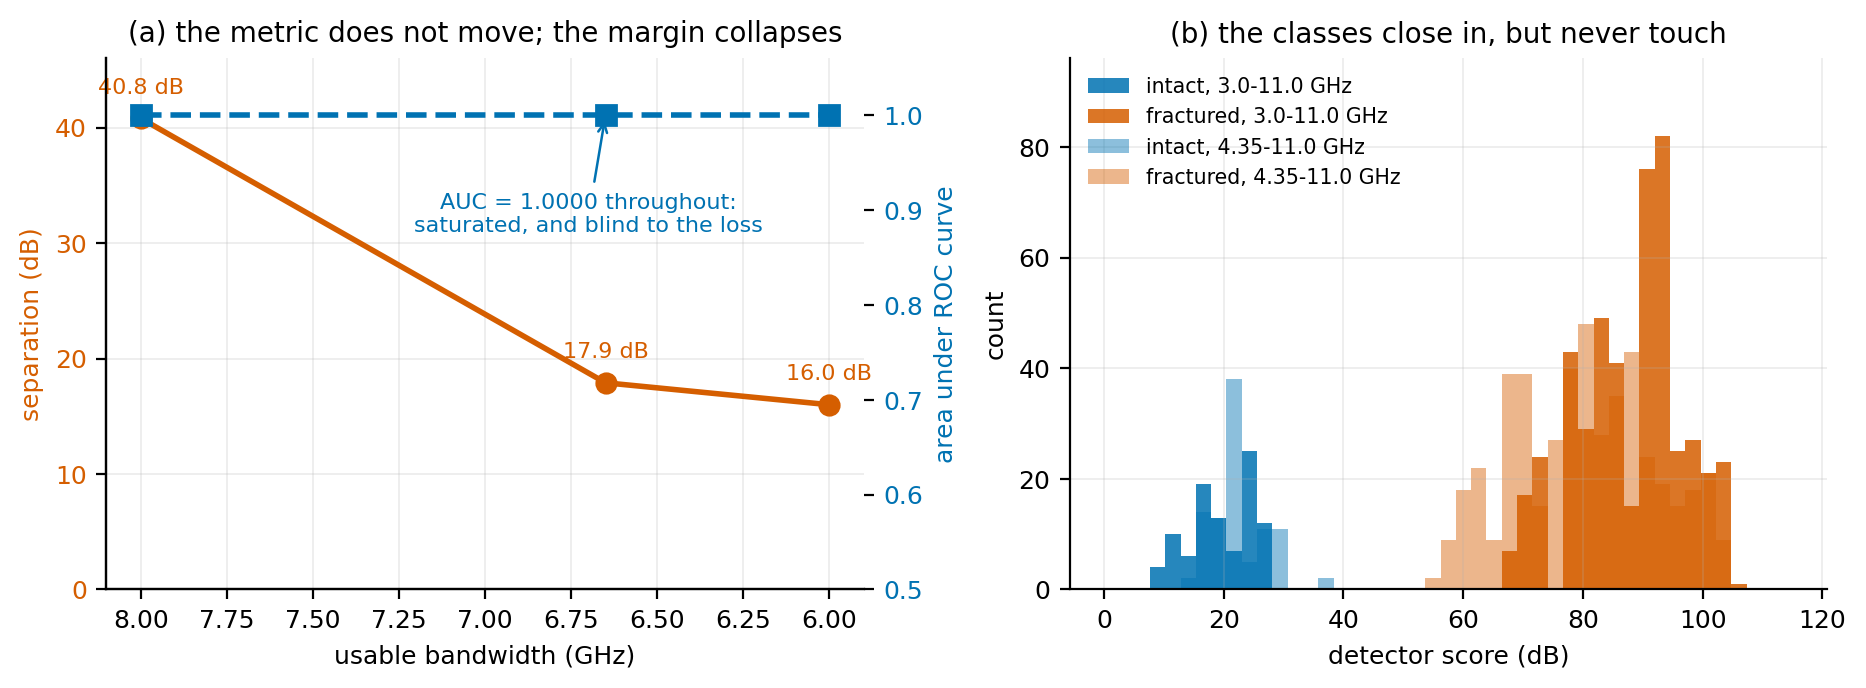
\includegraphics[width=0.92\textwidth]{figures/auc_saturation.png}
\caption{(a)~As usable bandwidth falls, the class separation collapses from
40.8\,dB to 16.0\,dB while the AUC remains pinned at 1.0000. (b)~The
underlying distributions converge from both sides but do not overlap, which
is precisely why the classification statistic cannot see the change.}
\label{fig:sat}
\end{figure*}

Every solved cell stores the full-band response, so the entire matrix can be
re-scored over a restricted window with no further electromagnetic
simulation. Bandwidth is thus varied with the geometry, the error model, the
processing chain and the detector all held exactly constant.

Table~\ref{tab:band} and Fig.~\ref{fig:sat} give the result. Removing
3.00--4.35\,GHz costs \textbf{22.9\,dB, more than half the total
separation}. The AUC is 1.0000 in all three windows and registers none of
it.

\subsection{Mechanism}
Band limitation degrades both classes, and the intact class is the more
damaging. The weakest fractured score falls from 68.5 to 55.7\,dB, as
expected from reduced penetration and resolution. The strongest
\emph{intact} score \emph{rises} from 27.7 to 37.8\,dB, which is a false
alarm rather than a missed detection. It occurs on one specimen at 6\,mm
overlay against a group mean of 23.7\,dB.

The mechanism follows from the resolution column of Table~\ref{tab:band}.
Bandwidth buys range resolution. At full bandwidth, migration resolves that
specimen's layered-interface reflection and collapses it; band-limited, the
artefact smears into the detection window and registers as a target. Because
the effect is specimen-dependent, the concern is variance rather than the
mean shift: one specimen in eight spikes, and a larger cohort would be
expected to contain worse outliers.

\subsection{Consequence for the instrument}
This measurement was not academic. An antipodal Vivaldi antenna
\cite{gazit} designed in openEMS \cite{openems} initially matched
4.35--12.00\,GHz against a 3--11\,GHz target, and the shortfall had been
documented as an acceptable compromise on the strength of an unchanged AUC.
Table~\ref{tab:band} shows that compromise cost 22.9\,dB. Re-examining the
input impedance showed the shortfall was never a low-frequency cutoff: the
design was already matched at 2.225--2.725\,GHz, reaching $-33$\,dB, two
gigahertz below its stated band edge. What lay between was a mismatch, a
resistive plateau of 24--37\,$\Omega$ across 3.25--4.40\,GHz. A load of
24.4\,$\Omega$ into a 50\,$\Omega$ feed predicts $-9.3$\,dB return loss and
$-9.14$\,dB was measured.

A tapered feed, 4.5\,mm at the flare and 1.74\,mm at the port, moved the
match to 2.48--12.00\,GHz, covering 99.69\,\% of the design band with a
worst in-band value of $-9.98$\,dB and a median input resistance of
45.6\,$\Omega$. Peak gain is 7.02, 11.87, 12.49, 12.06 and 9.33\,dBi at 3,
5, 7, 9 and 11\,GHz respectively; the 8--10\,dBi target is met from
approximately 4\,GHz upward and is not met at 3\,GHz, where the aperture is
0.6 wavelengths.

\subsection{Exposure}
The band straddles a boundary in current guidelines: specific absorption
rate applies below 6\,GHz and absorbed power density above it
\cite{icnirp,c951}. Both were evaluated for a layered limb at 12\,mm
standoff, with tissue densities from \cite{itis}. At the specified 0\,dBm
transmit power and worst-case illumination, all limits pass with a minimum
margin of 18$\times$; the binding quantity is absorbed power density above
6\,GHz.

\section{Discussion}

A saturated statistic is a lower bound, not a measurement. The defensible
claim from Table~\ref{tab:dist} is that under the modelled error budget the
classes separate by 40.8\,dB with no overlap, not that detection is perfect.
The binding assumption is the error model rather than the physics: a
physical bench adds cable flex, connector repeatability, operator variation
and genuine inter-specimen heterogeneity, none of which are simulated. The
40.8\,dB margin is the budget those unmodelled terms must consume before the
conclusion changes, and that framing is only available because the margin
was reported.

The practical consequence is concrete. Judged by AUC alone, the initial
antenna was adequate: the statistic did not move. Judged by margin, it cost
more than half the available budget, which is what motivated the redesign
reported above. The same reasoning applies to any design decision evaluated
against a saturated metric, including grid refinement, averaging time and
dynamic range.

We therefore suggest that studies reporting near-perfect classification also
report the separation between classes in the detector's own units, together
with the extreme values of each class. This costs nothing, is not an
additional experiment, and distinguishes a comfortable result from a
marginal one in exactly the regime where the classification statistic
cannot.

\section{Limitations}

\begin{enumerate}
\item The injected error model is the binding assumption. A physical bench
adds terms this work does not model.
\item Every fracture is at a known position; the study measures
separability, not localisation.
\item Propagation is two-dimensional TM$_z$. A three-dimensional
cylindrical model has been implemented and verified against the solver but
the comparison is not yet run, so no claim is made about the effect of
curvature or out-of-plane scattering.
\item Eight simulated specimens are not eight cadaveric bones.
\item The imaging model excites with an elementary dipole, not the antenna
of Section~III-D; antenna and imaging results are independent.
\item Antenna gain at 3\,GHz is unmet, and was shown not to be reachable by
resizing within the specified board.
\item Exposure is assessed by calculation, which is not a substitute for
measurement to IEC 62209.
\end{enumerate}

No hardware was built and no human or animal subject was exposed at any
point in this work.

\section{Conclusion}

Across 192 full-wave acquisitions from eight simulated specimens, fractured
and intact limbs separate by 40.8\,dB with no overlap, giving an AUC of
1.0000 with leave-one-specimen-out sensitivity 0.998 and specificity 1.000.
Restricting the usable band removed more than half of that separation while
the AUC remained exactly 1.0000, and the mechanism is a loss of range
resolution that converts a resolvable layered-interface artefact into a
specimen-dependent false alarm. A perfect classification score is therefore
a ceiling rather than a result, and should be accompanied by the margin it
conceals.

All code, data-generating scripts and figures are available at
\url{https://github.com/amalnathkp13-boop/bone-fracture-rf-sensing}.

%% ===================================================================
%% REFERENCES
%%
%% The eight entries below are the works this study actually rests on
%% and have been checked. Before submission you MUST add recent
%% domain-specific references on microwave imaging of bone -- a
%% reviewer will expect prior art for the application itself, not only
%% for the tools. Suggested searches: "microwave imaging bone",
%% "UWB bone fracture detection", "microwave tomography bone density".
%% Place them in the Introduction where prior simulation studies are
%% mentioned.
%% ===================================================================
\begin{thebibliography}{00}

\bibitem{gabriel}
S.~Gabriel, R.~W. Lau, and C.~Gabriel, ``The dielectric properties of
biological tissues: III. Parametric models for the dielectric spectrum of
tissues,'' \emph{Phys. Med. Biol.}, vol.~41, no.~11, pp.~2271--2293, 1996.

\bibitem{gprmax}
C.~Warren, A.~Giannopoulos, and I.~Giannakis, ``gprMax: Open source software
to simulate electromagnetic wave propagation for Ground Penetrating Radar,''
\emph{Comput. Phys. Commun.}, vol.~209, pp.~163--170, 2016.

\bibitem{openems}
T.~Liebig, A.~Rennings, S.~Held, and D.~Erni, ``openEMS -- a free and open
source equivalent-circuit (EC) FDTD simulation platform,'' \emph{Int. J.
Numer. Model.}, vol.~26, no.~6, pp.~680--696, 2013.

\bibitem{gazit}
E.~Gazit, ``Improved design of the Vivaldi antenna,'' \emph{IEE Proc. H},
vol.~135, no.~2, pp.~89--92, 1988.

\bibitem{icnirp}
International Commission on Non-Ionizing Radiation Protection, ``Guidelines
for limiting exposure to electromagnetic fields (100 kHz to 300 GHz),''
\emph{Health Phys.}, vol.~118, no.~5, pp.~483--524, 2020.

\bibitem{c951}
\emph{IEEE Standard for Safety Levels with Respect to Human Exposure to
Electric, Magnetic, and Electromagnetic Fields, 0 Hz to 300 GHz}, IEEE Std
C95.1-2019, 2019.

\bibitem{itis}
P.~A. Hasgall \emph{et al.}, ``IT'IS database for thermal and
electromagnetic parameters of biological tissues,'' Version 4.1, 2022.

\bibitem{bh}
Y.~Benjamini and Y.~Hochberg, ``Controlling the false discovery rate: a
practical and powerful approach to multiple testing,'' \emph{J. R. Stat.
Soc. B}, vol.~57, no.~1, pp.~289--300, 1995.

\end{thebibliography}

\end{document}
